\documentclass[10pt]{beamer}

\usepackage[vlined,english]{algorithm2e}
\DontPrintSemicolon

\usepackage{graphicx}
\usepackage[normalem]{ulem}
\usepackage{color,soul}
\usepackage{multirow}
\usepackage{tikz}
\usetikzlibrary{decorations.pathreplacing}
\usetikzlibrary{calc}
\usetikzlibrary{positioning}
\usetikzlibrary{arrows.meta}
\usetikzlibrary{shapes}
\usetheme[numbering=fraction,titleformat=smallcaps,progressbar=frametitle]{metropolis}
\usepackage[normalem]{ulem}

\usepackage{svg}

\usepackage[binary-units,group-digits,group-separator={,}]{siunitx}
\DeclareSIUnit\flop{Flop}
\DeclareSIUnit\flops{\flop\per\second}
\newcommand{\Num}[1]{\num[group-separator={,}]{#1}\xspace}
\newcommand{\NSI}[2]{\SI[group-separator={,}]{#1}{#2}\xspace}


% From https://github.com/matze/mtheme/issues/237#issuecomment-258718692
\makeatletter
\setlength{\metropolis@titleseparator@linewidth}{1.5pt}
\setlength{\metropolis@progressonsectionpage@linewidth}{1.5pt}
\setlength{\metropolis@progressinheadfoot@linewidth}{1pt}
\makeatother

\usepackage{fontawesome}

\newcommand{\backupbegin}{
   \newcounter{framenumberappendix}
   \setcounter{framenumberappendix}{\value{framenumber}}
}
\newcommand{\backupend}{
   \addtocounter{framenumberappendix}{-\value{framenumber}}
   \addtocounter{framenumber}{\value{framenumberappendix}}
}

% Command to make the last slide, which shows copies of the other slides
\newcommand{\addframe}[1] {\includegraphics[page=#1, width=0.3\textwidth]{slides_old.pdf}}

% *** SPECIFIC MACROS ***
% specific macro definition for the paper
%
% requires amsthm, xspace

% theorem-like environment
\newtheorem{thm}{Theorem}
\newtheorem{lem}[thm]{Lemma}
\newtheorem{prop}{Proposition}
\newtheorem{propty}{Property}
\newtheorem{defn}{Definition}

% asymptotic complexity (Landau) notations
\newcommand{\landauO}{\ensuremath{\mathcal{O}}\xspace}
\newcommand{\landauOmega}{\ensuremath{\Omega}\xspace}
\newcommand{\landauTheta}{\ensuremath{\Theta}\xspace}
\newcommand{\landauo}{\ensuremath{o}\xspace}
\newcommand{\landauomega}{\ensuremath{\omega}\xspace}
\newcommand{\landauorder}{\ensuremath{\sim}\xspace}

% scheduling notations
\newcommand{\graham}[3]{\mbox{\ensuremath{#1\mid#2\mid#3}}}
\newcommand{\Cmax}{\ensuremath{C_{\max}}\xspace}

% complexity classes
\newcommand{\cNP}{\textbf{NP}\xspace}  % bold notations
\newcommand{\cP}{\textbf{P}\xspace}
% \newcommand{\cNP}{\ensuremath{\mathcal{N\!P}}\xspace}  % round notations
% \newcommand{\cP}{\ensuremath{\mathcal{P}}\xspace}

% Machine states
\newcommand{\computing}{computing}
\newcommand{\idle}{idle}
\newcommand{\off}{of\!f}
\newcommand{\on}{on}
\newcommand{\ontooff}{\on\rightarrow\off}
\newcommand{\offtoon}{\off\rightarrow\on}

% CCGRID 2017
\newcommand{\ra}[1]{\renewcommand{\arraystretch}{#1}}

% Cluster 2017
\newcommand{\overbar}[1]{\mkern 1.5mu\overline{\mkern-1.5mu#1\mkern-1.5mu}\mkern 1.5mu}

\newlength\mylen % algorithm2e hack
\newcommand\myinput[1]{%
  \settowidth\mylen{\KwIn{}}%
  \setlength\hangindent{\mylen}%
  \hspace*{\mylen}#1\\}

\newcommand\myoutput[1]{% algorithm2e hack
  \settowidth\mylen{\KwOut{}}%
  \setlength\hangindent{\mylen}%
  \hspace*{\mylen}#1\\}



%%%%%%%%%%%%%%%%%%%%%%%
% Modular compilation %
%%%%%%%%%%%%%%%%%%%%%%%
\newif\ifwatermark
\watermarktrue

\newif\iftotalcompilation
\totalcompilationtrue

\newcommand{\inputchapter}[2]{%
  \ifdef{#1}%
    {\input{#2}\cleardoublepage}%
    {}%
}

% Modeling notations
\newcommand{\model}[2][]{\ensuremath{\bm{M}_{#1}\ifthenelse{\equal{#2}{}}{}{\!-\!}{#2}}\xspace}
\newcommand{\modelp}[2][]{\ensuremath{\bm{M'}_{#1}\!\ifthenelse{\equal{#2}{}}{}{\!-\!}{#2}}\xspace}
\newcommand{\noise}[2][]{\ensuremath{\bm{N}_{#1}\ifthenelse{\equal{#2}{}}{}{\!-\!}{#2}}\xspace}
\newcommand{\noisep}[2][]{\ensuremath{\bm{N'}_{#1}\!\ifthenelse{\equal{#2}{}}{}{\!-\!}{#2}}\xspace}
\newcommand{\norm}{\ensuremath{\mathcal{N}}\xspace}
\newcommand{\mcdots}{\ensuremath{\!\cdot\!\cdot\!\cdot\!}\xspace}
\newcommand{\unif}[2]{\ensuremath{\mathcal{U}\left({#1},{#2}\right)}\xspace}

% Abreviations
\newcommand{\eg}{e.g.\@\xspace}
\newcommand{\ie}{i.e.\@\xspace}
\newcommand{\aka}{a.k.a.\@\xspace}
\newcommand{\resp}{resp.\@\xspace}
\newcommand{\etal}{et~al.\@\xspace}
\newcommand{\dgemm}{\texttt{dgemm}\@\xspace}
\newcommand{\recv}{\texttt{MPI\_Recv}\@\xspace}
\newcommand{\send}{\texttt{MPI\_Send}\@\xspace}
\newcommand{\isend}{\texttt{MPI\_Isend}\@\xspace}
\newcommand{\iprobe}{\texttt{MPI\_Iprobe}\@\xspace}
\newcommand{\pyce}{\texttt{pycewise}\@\xspace}

% Referencing several times a footnote
% See https://tex.stackexchange.com/a/54240
\newcommand{\savefootnote}[2]{\footnote{\label{#1}#2}}
\newcommand{\repeatfootnote}[1]{\textsuperscript{\ref{#1}}}


\definecolor{darkgray}{HTML}{333333}
\definecolor{gray}{HTML}{4D4D4D}
\definecolor{lightgray}{HTML}{BBBBBB}
\definecolor{green}{HTML}{C2E15F}
\definecolor{orange}{HTML}{FDA333}
\definecolor{purple}{HTML}{D3A4F9}
\definecolor{red}{HTML}{FB4485}
\definecolor{blue}{HTML}{6CE0F1}
\definecolor{pblue}{HTML}{0395DE}
\definecolor{materialpurple}{HTML}{9C27B0}
\definecolor{materialindigo}{HTML}{3F51B5}
\definecolor{materialblue}{HTML}{2196F3}
\definecolor{materialcyan}{HTML}{00BCD4}
\definecolor{materialteal}{HTML}{009688}
\definecolor{materialgreen}{HTML}{4CAF50}
\definecolor{materiallime}{HTML}{CDDC39}
\definecolor{materialamber}{HTML}{FFC107}
\definecolor{materialbrown}{HTML}{795548}
\definecolor{materialred}{HTML}{FF4436}
\definecolor{materialorange}{HTML}{FF5722}
\setbeamercolor{normal text}{bg=white}
\colorlet{mycolor}{materialblue}
\setbeamercolor{alerted text}{fg=mycolor}

%\renewcommand{\emph}[1]{\SoulColor{lightorange}\hl{#1}}
%\makeatletter
%\let\HL\hl
%\renewcommand\hl{%
%  \let\set@color\beamerorig@set@color
%  \let\reset@color\beamerorig@reset@color
%  \HL}
%\colorlet{mycolorlight}{mycolor!30}
%\sethlcolor{mycolorlight}
%\makeatother
%\renewcommand<>{\hl}[1]{\only#2{\beameroriginal{\hl}}{#1}}
%\renewcommand<>{\emph}[1]{\only#2{\beameroriginal{\hl}}{#1}}


\setlength{\interspacetitleruled}{0pt}%
\setlength{\algotitleheightrule}{0pt}%

% Using a small font for verbatim blocks
\def\changefont#1{%
  \setbeamertemplate{itemize/enumerate body begin}{#1}
  \setbeamertemplate{itemize/enumerate subbody begin}{#1}
  #1}
\makeatletter
\newcommand{\verbatimfont}[1]{\renewcommand{\verbatim@font}{\ttfamily#1}}
\makeatother
\verbatimfont{\scriptsize}%small
\let\endmintedbak=\endminted
\def\endminted{\endmintedbak\vspace{-1cm}}


\date{}
\author{\textbf{Tom Cornebize}}
\date{2 June 2021, PhD defense}
\title{High Performance Computing: Towards Better Performance Predictions and Experiments}

\begin{document}
\titlegraphic{
    \begin{picture}(0,0)
        \put(310,-200){\makebox(0,0)[rt]{
            \begin{minipage}{\textwidth}
                \includesvg[height=1cm]{img/logo_uga.svg}\hfill%
                
\includegraphics[height=1cm]{img/slides/logo_cnrs.png}\hfill%
                
\includegraphics[height=1cm]{img/slides/logo_inria.png}
            \end{minipage}
        }}
    \end{picture}
}

\maketitle

\begin{frame}{No science without computing}
    \begin{columns}
        \begin{column}[c]{.33\columnwidth}
            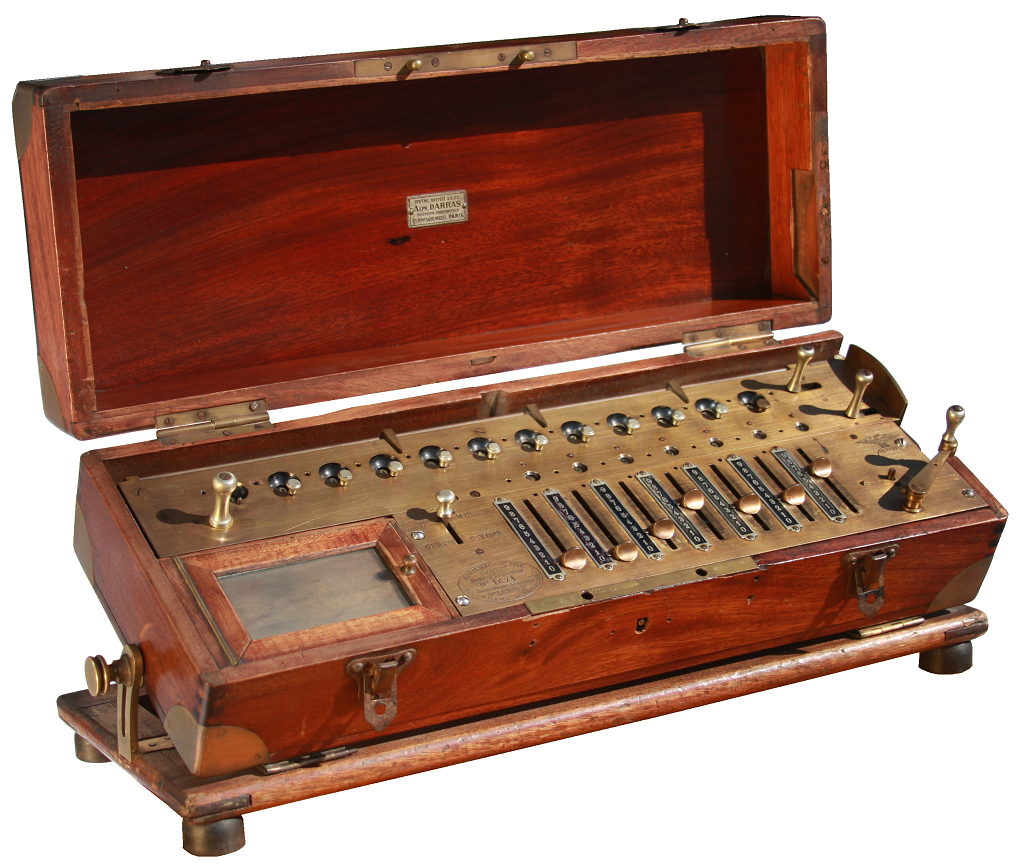
\includegraphics[width=\linewidth]{img/slides/arithmometer.png}
            Arithmomètre (1851)
        \end{column}
        \begin{column}[c]{.33\columnwidth}
            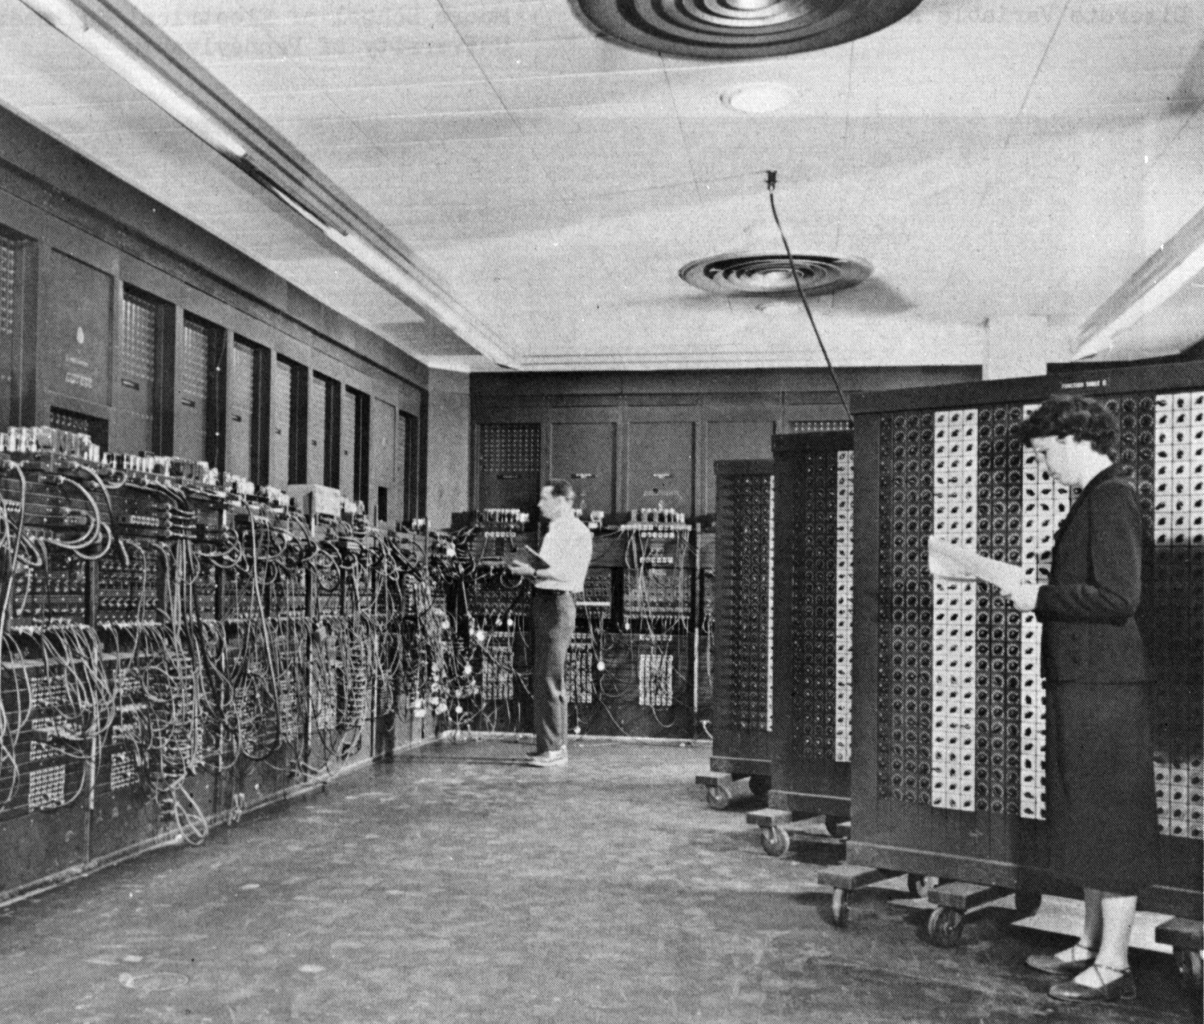
\includegraphics[width=\linewidth]{img/slides/eniac.jpg}
            ENIAC (1945)
        \end{column}
        \begin{column}[c]{.33\columnwidth}
            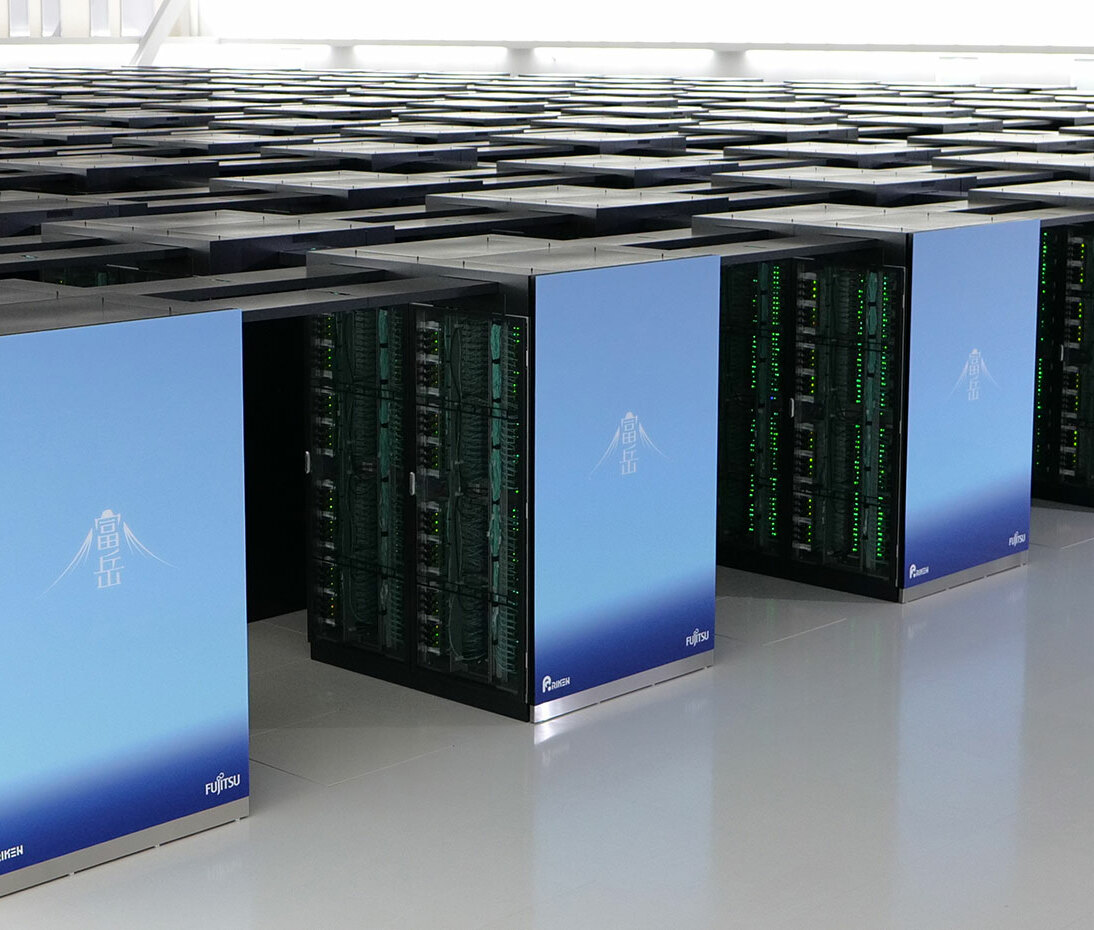
\includegraphics[width=\linewidth]{img/slides/fugaku.jpg}
            Fugaku (2021)
        \end{column}
    \end{columns}
    \vfill

    \pause

    Last decades:
    \begin{itemize}
        \item Exponential \alert{performance} improvements
        (\eg sequencing an entire human genome costed \SI{100000000}[\$]{} in 2001, \SI{1000}[\$]{} now)
        \item At the price of \alert{complexity} (both software and hardware)
    \end{itemize}
\end{frame}

\begin{frame}{Experimental study of computer performance}
    \begin{columns}
        \begin{column}[c]{.5\columnwidth}
            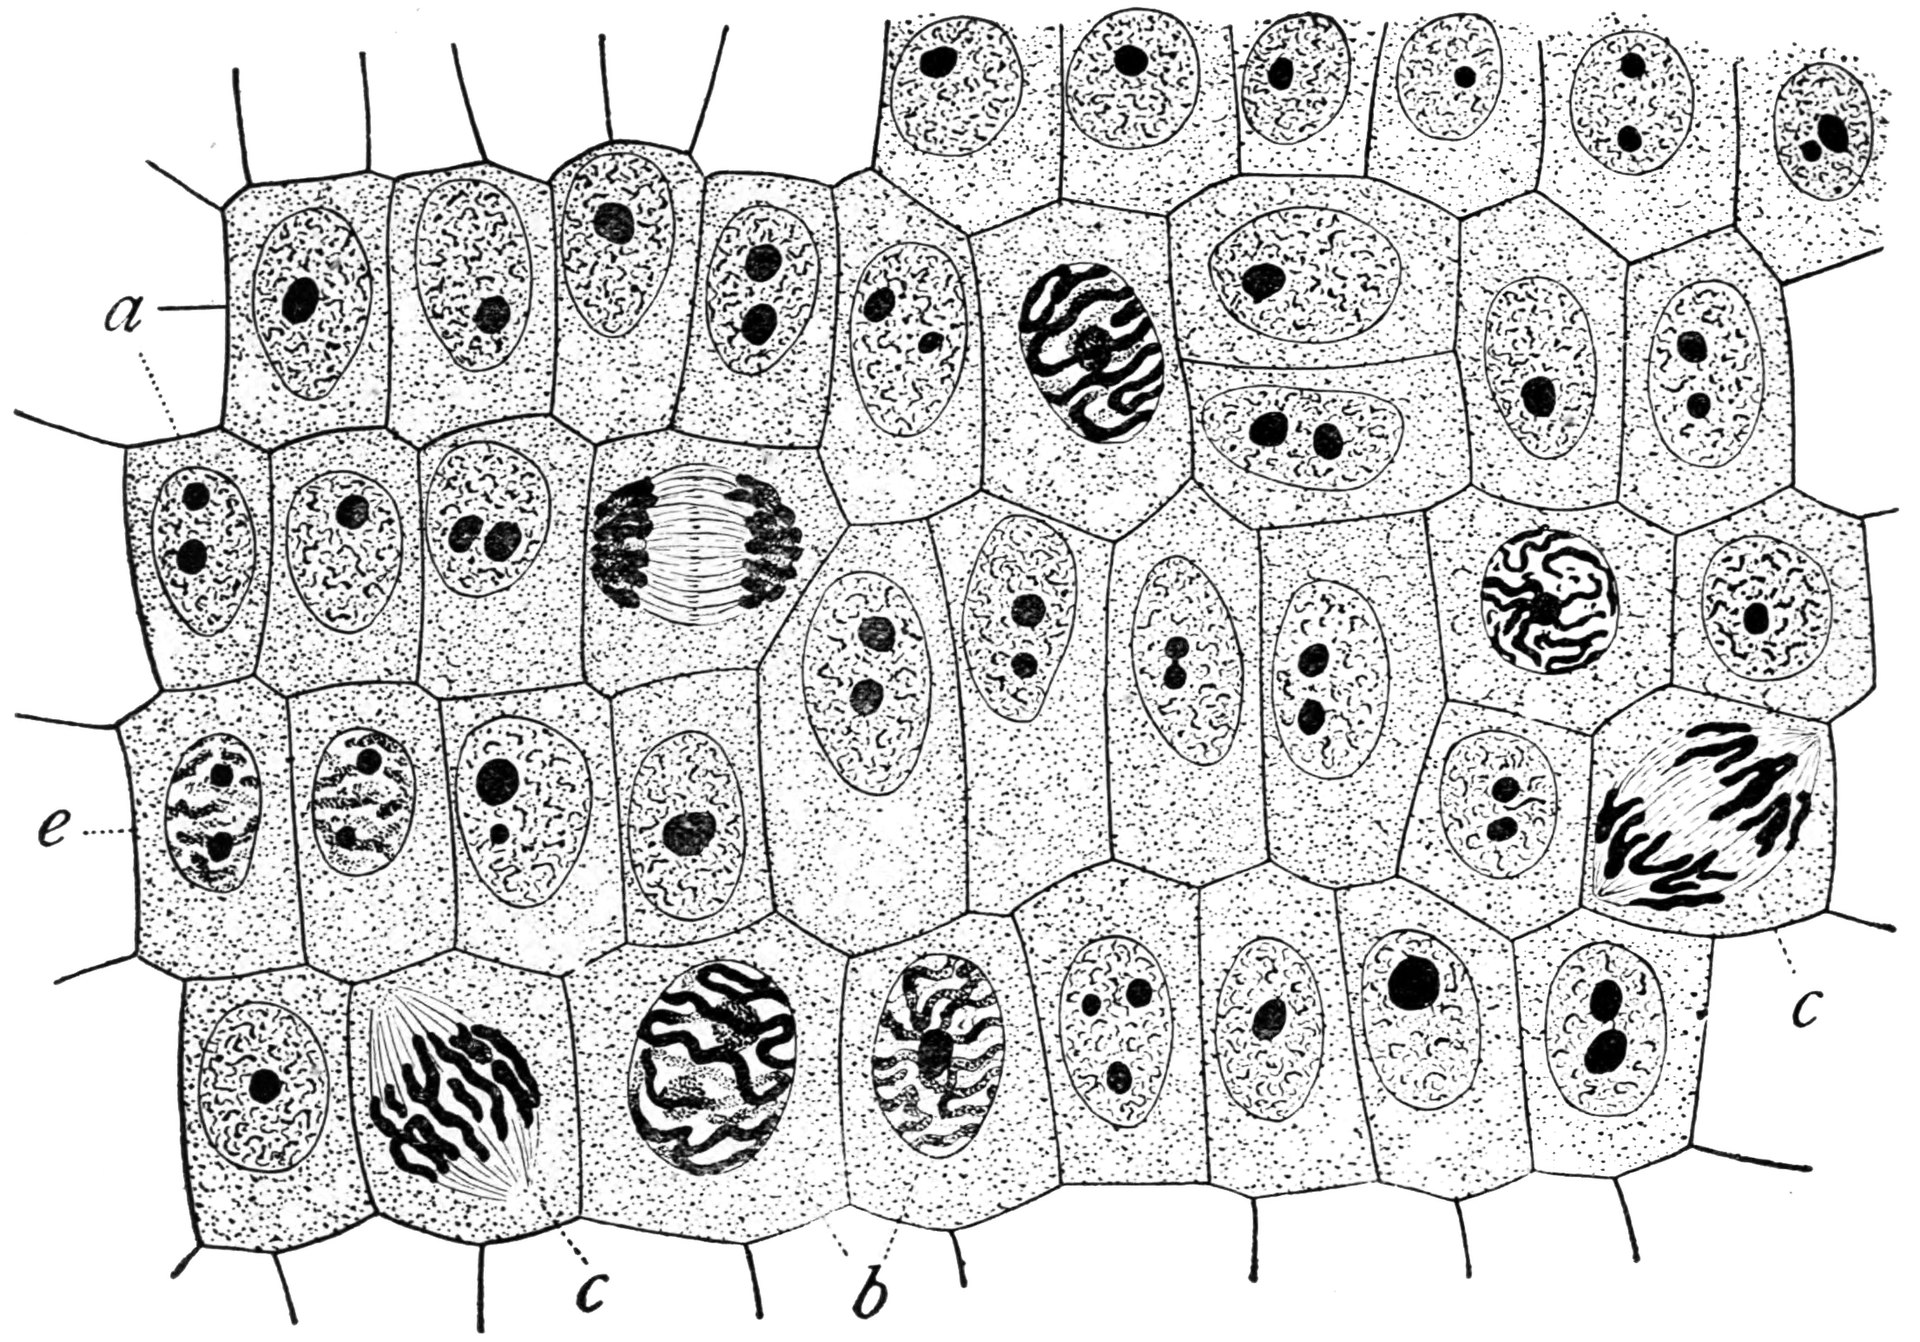
\includegraphics[width=\linewidth]{img/slides/cells.jpg}
        \end{column}
        \begin{column}[c]{.5\columnwidth}
            Similar to natural sciences
            \begin{flalign*}
                \text{Complexity} &\Rightarrow \text{Variability and Opacity}&\\
                                  &\Rightarrow \text{No perfect model}&\\
                                  &\Rightarrow \text{Need for \alert{experiments}}&\\
            \end{flalign*}
        \end{column}
    \end{columns}
    \pause
    \vfill
    Empirical studies can be carried in \alert{reality} or in \alert{simulation}
\end{frame}

\begin{frame}{Context}
    \textbf{Typical Performance Evaluation Questions} (Given my application and a supercomputer)

    \begin{minipage}[m]{0.35\linewidth}
        
\includegraphics[width=\textwidth]{img/slides/computer_guy_meme.pdf}
    \end{minipage} %
    \begin{minipage}[m]{0.64\linewidth}
    \begin{itemize}
        \item \textbf{Before} running
        \begin{itemize}
            \item How many nodes?
            \item For how long?
            \item Which parameters?
        \end{itemize}
        \pause
        \item \textbf{After} running
        \begin{itemize}
            \item Performance as ``expected''?
            \item Problem in the app or the platform?
        \end{itemize}
    \end{itemize}
    \end{minipage}
    \pause

    \begin{center}
        So many large-scale runs, solely to tune performance?!?
    \end{center}

    \pause

    \textbf{Holy Grail: Predictive Simulation on a ``Laptop''}

    Capture the \textbf{whole application}  and \textbf{platform complexity}
\end{frame}

\begin{frame}[plain]
    \onslide<+->
    \begin{LARGE}
        Initial goal: \alert{\textbf{predict}} the performance of a parallel application
    \end{LARGE}
    \vfill
    \onslide<+->
    \begin{block}{Thesis contributions (towards this goal)}
        \begin{itemize}
            \item Case study: High Performance Linpack (HPL)
            \item Extensive (in)validation, comparing simulations with reality
            \item Demonstrate it is possible to \alert{predict faithfully} the behavior of complex parallel applications
            \item Modeling correctly the platform variability is key
        \end{itemize}
    \end{block}
    \onslide<+->
    \begin{block}{Thesis contributions (made on the way)}
        \begin{itemize}
            \item \textcolor<+->{lightgray}{Automation (of experiments, statistical analyzes, etc.)}
            \item \textcolor<.>{lightgray}{Experiment methodology, to bias or not to bias}
            \item Performance tests, to detect eventual platform changes
        \end{itemize}
    \end{block}
\end{frame}

\section{Performance prediction through simulation}%

\begin{frame}[fragile]{Sim(Em)ulation: The SMPI Approach}
    \begin{columns}
        \begin{column}[c]{.2\columnwidth}
            \scalebox{.8}{\begin{tikzpicture}[xscale=1,yscale=1]
                \node (nodehost) [name=nodehost]
                { 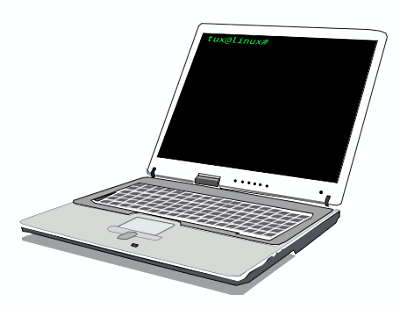
\includegraphics[height=23mm]{img/slides/laptop.png}};

                %\node (nodelisting) [above right= -25mm of nodehost]%, overlay]
                % { \includegraphics[height=12mm]{fig/mpi-codelisting.png}};

                \node (nodeimagine) [
                    shape             = cloud callout,
                    cloud puffs       = 11,
                    aspect            = 1.5,
                    opacity           =.75,
                    draw              = black!90!white, % colour of the border
                    top color         = white,                % | filling of the node
                    bottom color      = black!30!white, % |
                    text              = black!90!white, % colour of the fonts
                    thick,                              % thickness of the border
                    above             = 5mm of nodehost,
                    minimum height    = 25mm,
                    minimum width     = 30mm,
                    callout pointer shorten=7mm,
                    callout absolute pointer={(285:5mm)},%(nodelisting.northwest)},%(285:5.5mm)},
                ]{};

                \node at (nodeimagine) {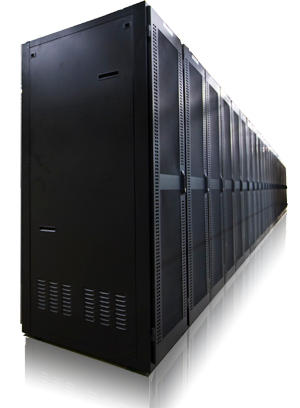
\includegraphics[width=15mm]{img/slides/cluster.png}};
            \end{tikzpicture}}
        \end{column}

        \begin{column}[c]{.85\columnwidth}
            \begin{picture}(0, 0)
                \put(170,-32){\hbox{
                    
\includegraphics[width=2cm]{img/slides/simgrid_logo.pdf}
                }}
            \end{picture}
            \begin{block}{Full reimplementation of MPI on top of}% \alert{SimGrid}}
                \medbreak
                \begin{itemize}
                    \item C/C++/F77/F90 codes run \alert{unmodified out of the box}
                    \item Simply replace mpicc/mpirun by smpicc/smpirun
                \end{itemize}
            \end{block}
            \pause
            \begin{block}{Emulation: how?}
                \begin{itemize}
                    \item Application runs for real on a laptop
                    \item Communications are faked, good fluid network models
                    \item \alert{Performance model} for the target platform
                \end{itemize}
            \end{block}
        \end{column}
    \end{columns}
    \pause
    Validations of SMPI before this thesis: simple applications without any high performance tricks
\end{frame}

\begin{frame}[fragile]{Quick word on HPL}
    Contribution: predict accurately the performance of HPL

    \begin{minipage}[b][0.2\textheight][c]{.2\linewidth}
        
\includegraphics[width=\linewidth]{img/slides/top_500.pdf}
    \end{minipage} \hfill %
    \begin{minipage}[b][0.25\textheight][t]{0.78\linewidth}
        \begin{itemize}
            \item Computations and communication overlap (custom collectives)
            \item More representative of some HPC applications
            \item Well established, used for the Top500
        \end{itemize}
    \end{minipage}
    \vfill
    \pause

    \begin{center}
        \begin{minipage}[b][0.4\textheight][t]{0.25\linewidth}
            \begin{tikzpicture}[scale=0.2]
                \draw (0, 0) -- (0, 12) -- (12, 12) -- (12, 0) -- cycle;
                \foreach \i in {2}{
                    \draw [fill=lightgray] (\i, 0) -- (\i, 12-\i) -- (12, 12-\i) -- (12, 0) -- cycle;
                    \draw [fill=gray] (\i, 12-\i) -- (\i, 12-\i-1) -- (\i+1, 12-\i-1) -- (\i+1, 12-\i) -- cycle;
                    \draw[very thick, -latex] (\i,12-\i) -- (\i+2,12-\i-2);
                    \draw[<->] (\i, 12-\i+0.5) -- (\i+1, 12-\i+0.5) node [pos=0.5, yshift=+0.15cm] {\scalebox{.8}{\texttt{NB}}};
                }
                \foreach \i in {3}{
                    \draw [fill=white] (\i, 0) -- (\i, 12-\i) -- (12, 12-\i) -- (12, 0) -- cycle;
                    \draw (\i,12-\i) -- (\i,0);
                    \draw[very thick, -latex] (\i,12-\i) -- (\i+2,12-\i-2);
                }
                \draw[dashed] (0, 12) -- (12, 0);
                \node(L) at (2, 2) {\ensuremath{\boldsymbol{L}}};
                \node(U) at (10, 10) {\ensuremath{\boldsymbol{U}}};
                \node(A) at (8, 4) {\ensuremath{\boldsymbol{A}}};
                \draw[<->] (0, -0.5) -- (12, -0.5) node [pos=0.5, yshift=-0.3cm] {$N$};
            \end{tikzpicture}
        \end{minipage}
        \begin{minipage}[b][0.4\textheight][t]{0.36\linewidth}\footnotesize
            \begin{algorithm}[H]
                Allocate and initialize $A$\;
                \For{$k=N$ \textbf{to} $0$ \textbf{step} \texttt{NB}}{
                    Allocate the panel\;
                    Factor the panel\;
                    Broadcast the panel\;
                    Update the sub-matrix\;
                }
            \end{algorithm}
        \end{minipage} \hfill \pause%
        \begin{minipage}[b][0.4\textheight][t]{0.35\linewidth}\footnotesize
            \begin{block}{Tuning parameters}
                \begin{itemize}
                    \item Process grid
                    \item Block size
                    \item Broadcast algorithm
                    \item etc.
                \end{itemize}
                Hundreds of combinations
            \end{block}
        \end{minipage}
    \end{center}
    \pause
    \textbf{Contribution}: Skip the expensive computations (mostly \dgemm) and replace them by performance models
\end{frame}

\begin{frame}{Modeling Commputations}
    \begin{equation*}
        \texttt{dgemm}_{\uncover<3->{i}}(M,N,K) =
        \only<1-2>{\alpha.M.N.K}\uncover<3->{\underbrace{\alpha_i.M.N.K}_{\text{per host}}}
        \uncover<5->{+ \underbrace{\beta_i.M.N +  \gamma_i.N.K + \dots }_{\text{polynomial model}}}
        \uncover<6->{+ \underbrace{\norm(0,\alpha'_i.M.N.K + \dots)}_{\text{polynomial noise}}}
    \end{equation*}

    \begin{center}
        \begin{tabular}{p{0.45\textwidth}p{0.45\textwidth}}
            \uncover<3->{Different color $\Rightarrow$ different host} &
            \uncover<4->{For a particular host} \\

            \includegraphics<1>[width=\linewidth]{img/slides/dgemm_heterogeneity_calib_1.png} %
            \includegraphics<2>[width=\linewidth]{img/slides/dgemm_heterogeneity_calib_2.png} %
            \includegraphics<3->[width=\linewidth]{img/slides/dgemm_heterogeneity_calib_3.png} &

            \includegraphics<4>[width=\linewidth]{img/slides/dgemm_model_calib_1.png} %
            \includegraphics<5>[width=\linewidth]{img/slides/dgemm_model_calib_2.png} %
            \includegraphics<6->[width=\linewidth]{img/slides/dgemm_model_calib_3.png} \\

        \end{tabular}
    \end{center}
\end{frame}

\begin{frame}{Modeling Communications}
    \textbf{Hand-crafted non-blocking collective operations} intertwinned with computations

    \begin{minipage}[t][.7\textheight][t]{\textwidth}
        \begin{center}
            \includegraphics<2>[width=.9\linewidth]{img/prediction/modeling/network/mpi_calibration.png}
        \end{center}
    \end{minipage}
\end{frame}


\section{Validating the predictions}

\begin{frame}[fragile]{Internal behavior of the application}
    256 MPI ranks, interrupted after the $5^{\text{th}}$ iteration\medskip

    \newcommand{\ganttcaption}[2]{\rotatebox{90}{\hspace{.6cm}$\text{#1}\atop \text{#2}$\hspace{-1cm}}}%
    \begin{overlayarea}{\linewidth}{7cm}
        \begin{tabular}{c@{}c}
            \only<+->{\ganttcaption{\hspace{.3cm}Reality}{}          & 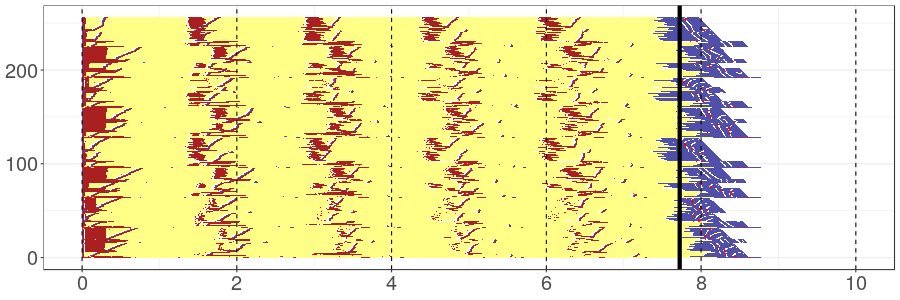
\includegraphics[width=.93\linewidth]{img/prediction/validation/traces/gantt_reality.png} \\}%
            \only<+>{\ganttcaption{Simple kernel}{Simple network}    & 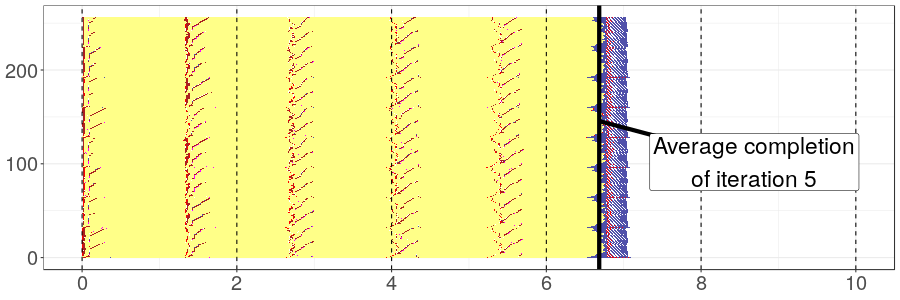
\includegraphics[width=.93\linewidth]{img/prediction/validation/traces/gantt_simulation_deterministic-CPU_linear-DGEMM_deterministic-network.png}\\}%
            \only<+>{\ganttcaption{Simple kernel}{Complex network}   & 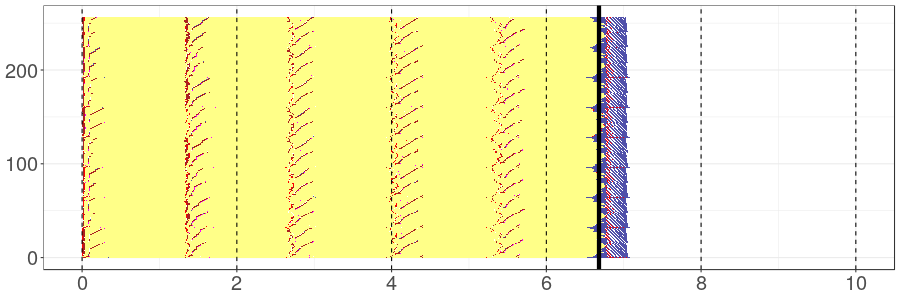
\includegraphics[width=.93\linewidth]{img/prediction/validation/traces/gantt_simulation_deterministic-CPU_linear-DGEMM_stochastic-network.png}\\}%
            \only<+>{\ganttcaption{Complex kernel}{Complex network}  & 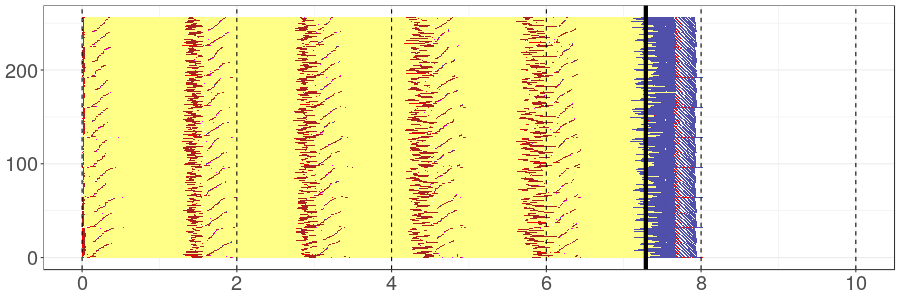
\includegraphics[width=.93\linewidth]{img/prediction/validation/traces/gantt_simulation_stochastic-CPU_polynomial-DGEMM_stochastic-network.png} \\}%
        \end{tabular}
    \end{overlayarea}
\end{frame}


\begin{frame}[fragile]{Influence of the problem size}
    Now the complete run, with 1024 MPI ranks

    \tikzstyle{model_label}=[anchor=south west, font=\scriptsize]
    \begin{tikzpicture}
        \node[anchor=south west,inner sep=0] at (0,0){
            \begin{minipage}{\linewidth}
                \includegraphics<1>[width=0.9\linewidth]{img/slides/validation_performance_1.pdf}
                \includegraphics<2>[width=0.9\linewidth]{img/slides/validation_performance_2.pdf}
                \includegraphics<3>[width=0.9\linewidth]{img/slides/validation_performance_3.pdf}
                \includegraphics<4->[width=0.9\linewidth]{img/slides/validation_performance_4.pdf}
            \end{minipage}
        };
        \onslide<3->{\draw[-latex] (9.7, 4.5) to[bend left] node [midway, right, model_label, anchor=west]
            {\textbf{Heterogeneity}} (9.7, 3.9) ;}
        \onslide<4->{\draw[-latex] (9.7, 3.9) to[bend left] node [midway, right, model_label,
            anchor=west]{\textbf{Variability}} (9.7, 3.5) ;}
    \end{tikzpicture}
    \onslide<5->{
        \textbf{Take-Away Message}: accurate prediction

        Modeling both \alert{spatial} and \alert{temporal} computation variability is essential
    }
\end{frame}

\begin{frame}{Influence of the geometry}
    \(P \times Q\) MPI processes, organized in a 2D grid

    \begin{center}
        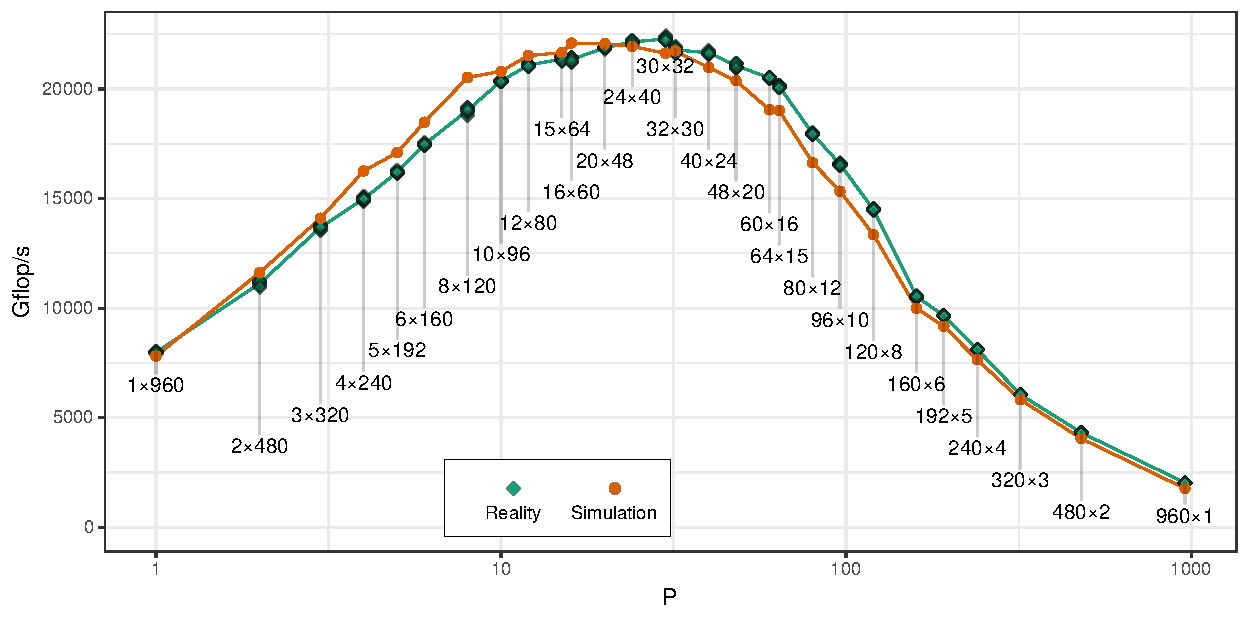
\includegraphics[width=0.9\linewidth]{img/slides/validation_geometry.pdf}
    \end{center}
\end{frame}

\begin{frame}{Influence of the other parameters}
    Tested the 72 combinations of the remaining parameters
    \begin{center}
        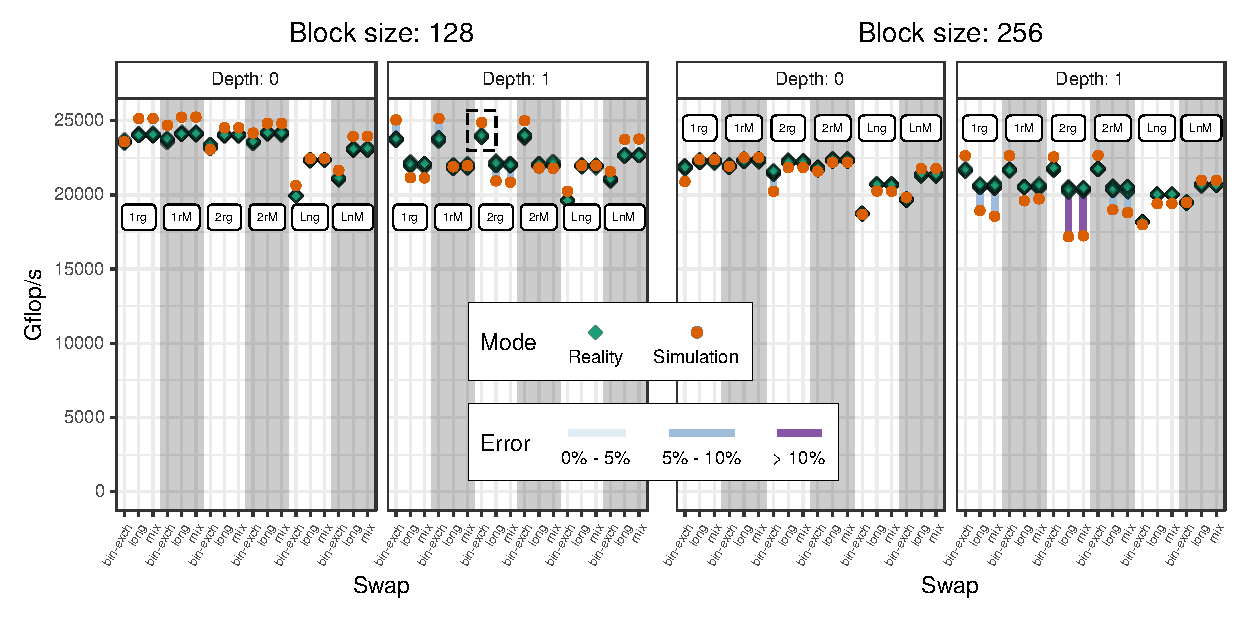
\includegraphics[width=0.9\linewidth]{img/prediction/validation/factorial/validation_factorial.pdf}
    \end{center}
\end{frame}

\begin{frame}[fragile]{Influence of a platform change}
    \tikzstyle{model_label}=[anchor=south west, font=\scriptsize]
    \begin{tikzpicture}
        \node[anchor=south west,inner sep=0] at (0,0){
            \begin{minipage}{\linewidth}
                \includegraphics<1>[width=0.9\linewidth]{img/slides/validation_temperature_1.pdf}
                \includegraphics<2>[width=0.9\linewidth]{img/slides/validation_temperature_2.pdf}
                \includegraphics<3->[width=0.9\linewidth]{img/slides/validation_temperature_3.pdf}
            \end{minipage}
        };
        \onslide<2->{\draw[-latex] (9.7, 4) to[bend left] node [midway, right, model_label, anchor=west]
            {\textbf{Overheating}} (9.7, 3.5) ;}
    \end{tikzpicture}
    \onslide<2->{On four nodes, the cooling system malfunctionned for several weeks}
    \vfill
    \onslide<4->{
        \textbf{Take-Away Message}: Re-measuring \dgemm durations to generate a new model was enough to account for the
        platform change
    }
\end{frame}

\begin{frame}{Use case: sensibility analysis}
    What if the network topology of my cluster was different?

    \begin{center}
        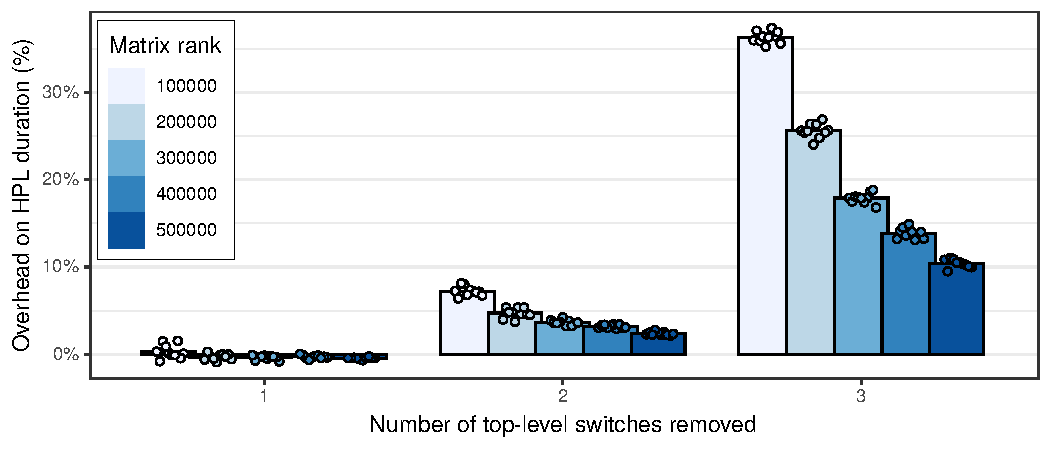
\includegraphics[width=0.9\linewidth]{img/prediction/sensibility/topology/whatif_removing_switches.pdf}
    \end{center}

    \pause
    \begin{flalign*}
        \text{Faithful surrogate} &\Rightarrow \text{Empirical studies of hypothetical platforms}&\\
                                  &\Rightarrow \text{Extrapolation of existing platforms}&\\
                                  &\Rightarrow \text{Accounting for spatial and temporal variability}&\\
    \end{flalign*}
\end{frame}

\begin{frame}[plain]
    \begin{LARGE}
        Goal: performance prediction~~~\alert{\textbf{\Huge \checkmark}}
    \end{LARGE}
    \medbreak
    \pause

    Main difficulties:
    \begin{itemize}
        \item Realistic experimental conditions
        \item Platform changes (\eg, the cooling issue)
    \end{itemize}
\end{frame}

\begin{frame}{Parenthesis: on the difficulties of experimentation}
    \alert{Experimental biases} when measuring \dgemm or MPI durations

    Effect on durations, but also other metrics (\eg CPU frequency)
    \onslide<+->
    \begin{itemize}[<+->]
        \item Sampling method for generating the sequence of calls\\
             \alert{\(\sim 10\%\)} systematic performance change
        \item Interferences between computations and communications\\
             \alert{\(\sim 50\%\)} performance change in extreme configurations
        \item Content of the matrices used by \dgemm\\
             \alert{\(\sim 5\%\)} systematic performance change
    \end{itemize}

    \onslide<+->
    Bias may be desirable in some situations
\end{frame}


\section{Performance tests}%

\begin{frame}{Regular measures}
    On a near-daily basis, run the \dgemm calibration code on
    \begin{picture}(0, 0)
        \put(-3, -11){\hbox{
            
\includegraphics[width=2cm]{img/slides/grid5000-logo.pdf}
        }}
    \end{picture}

    454 nodes (792 CPU) from 12 clusters
    \pause

    For each CPU, collect:
    \begin{itemize}
        \item average \dgemm performance
        \item \dgemm coefficients of regression (\ie the model for simulation)
        \pause
        \item average CPU frequency
        \item average CPU power consumption
        \item average DRAM power consumption
        \item average temperature
    \end{itemize}
    \pause
    If the platform did not change, then each parameter is \alert{normally~distributed} (thanks to CLT)
\end{frame}

\begin{frame}{Fluctuation interval}
    Given a sequence of \alert{old~observations} $x_1, \dots, x_n$ and a \alert{new~observation} $x_{n+1}$, how likely
    was it to observe $x_{n+1}$?

    \begin{minipage}{0.5\linewidth}
        \begin{center}
            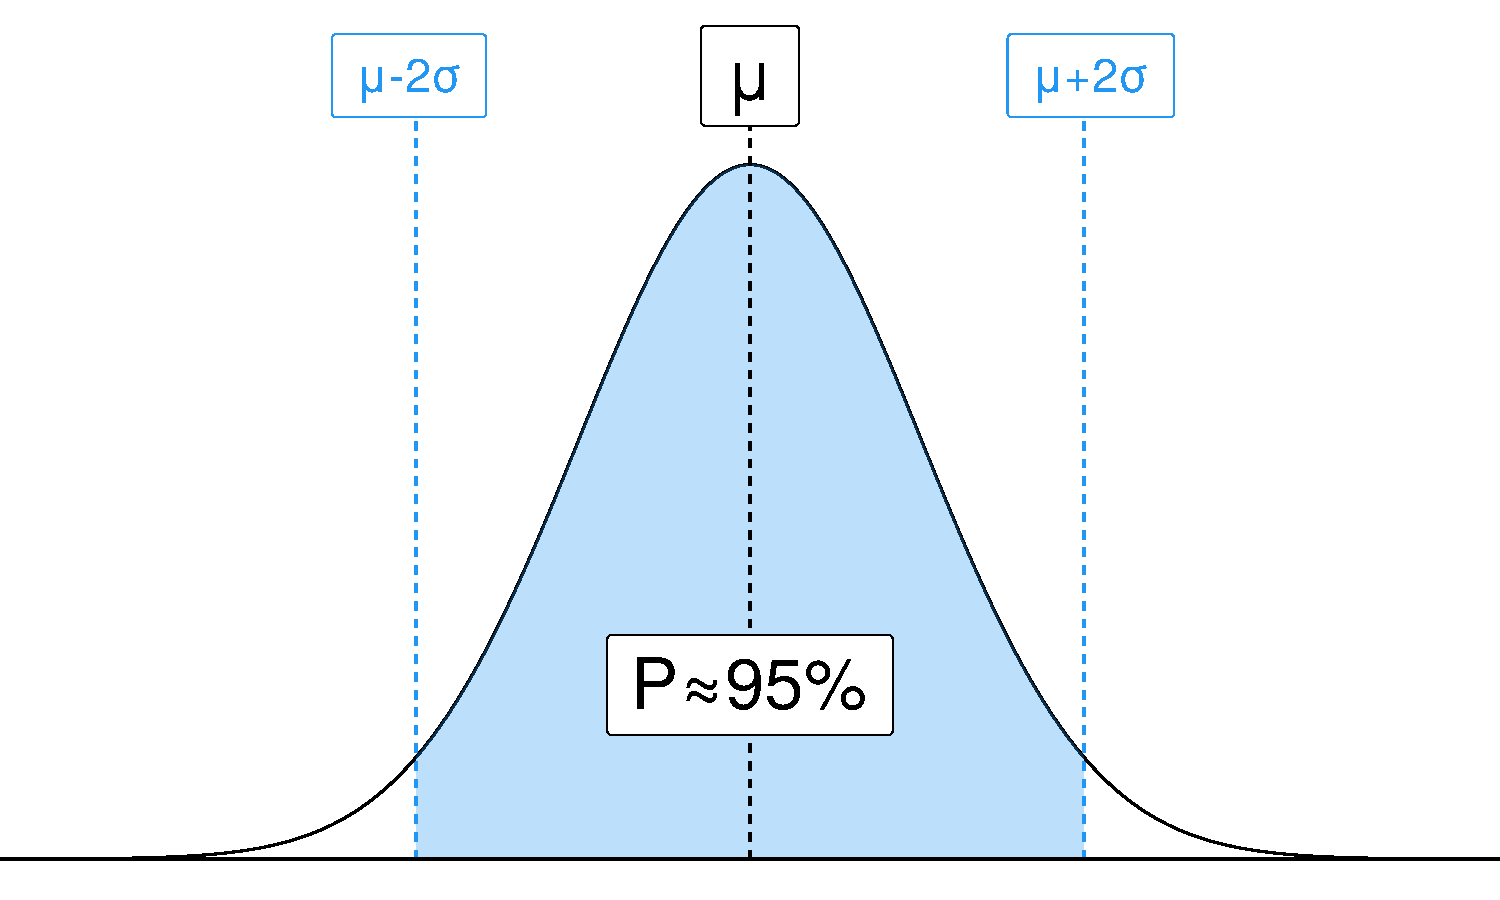
\includegraphics[width=\linewidth]{img/slides/normal.pdf}
        \end{center}
    \end{minipage}\hfill%
    \begin{minipage}{0.48\linewidth}
        Take the sample mean \(\bar x\) and standard deviation \(s\) of the old observations

        \medbreak

        \(\mathbb{P}\left(x_{n+1}\in\left[\bar x - 2s ; \bar x + 2s\right]\right) \approx 95\%\)
    \end{minipage}

    \pause
    Note: using the F distribution instead of the normal distribution\\
    (the \alert{true} mean and standard deviation are unknown)
\end{frame}

\begin{frame}{Fluctuation interval for several variables}
    With several variables, use their \alert{covariance~matrix}

    Example in dimension 2, with \(\mathbb{P}(x_{n+1} \in \text{interval}) \approx 99.5\%\)

    \begin{center}
        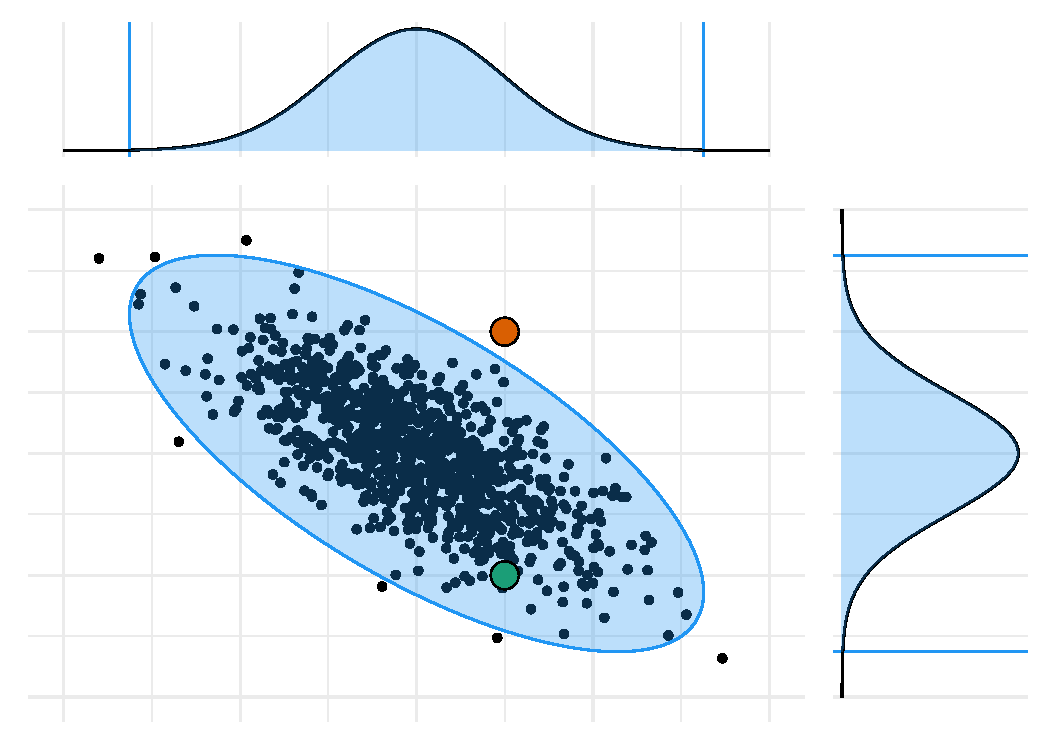
\includegraphics[width=0.8\linewidth]{img/experiment/non_regression/statistics/single_point.pdf}
    \end{center}
\end{frame}

\begin{frame}{Result: performance fluctuation}
    \begin{center}
        \begin{minipage}[t][.4\textheight][t]{\textwidth}
            Performance fluctuation of the node dahu-14\\
            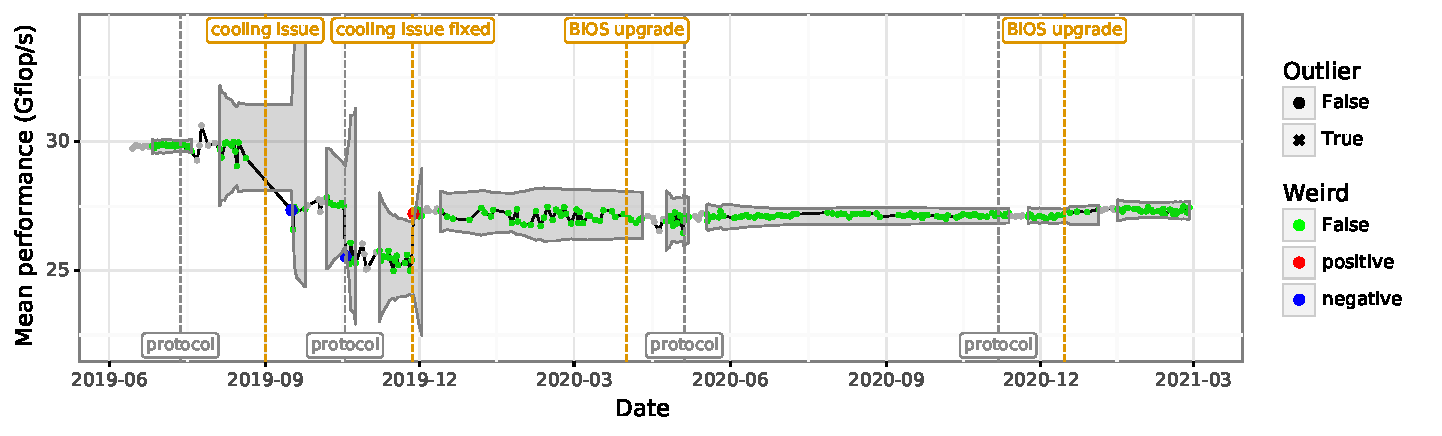
\includegraphics[width=0.9\linewidth]{img/slides/evolution_dahu-14.pdf}
        \end{minipage}
        \begin{minipage}[t][.4\textheight][t]{\textwidth}
            \uncover<2->{Performance fluctuation of the node dahu-32}\\
            \includegraphics<2>[width=0.9\linewidth]{img/slides/evolution_dahu-32.pdf}
        \end{minipage}
    \end{center}
\end{frame}

\begin{frame}{Fluctuation interval for several measures}
    How to detect more subtle changes? Take several consecutive measures \(x_{n+1},\dots,x_{n+k}\), use their
    \alert{average} and shrink the interval accordingly

    \onslide<2->{Example with 5 measures} \onslide<3->{(averages represented by crosses)}

    \begin{center}
        \only<2>{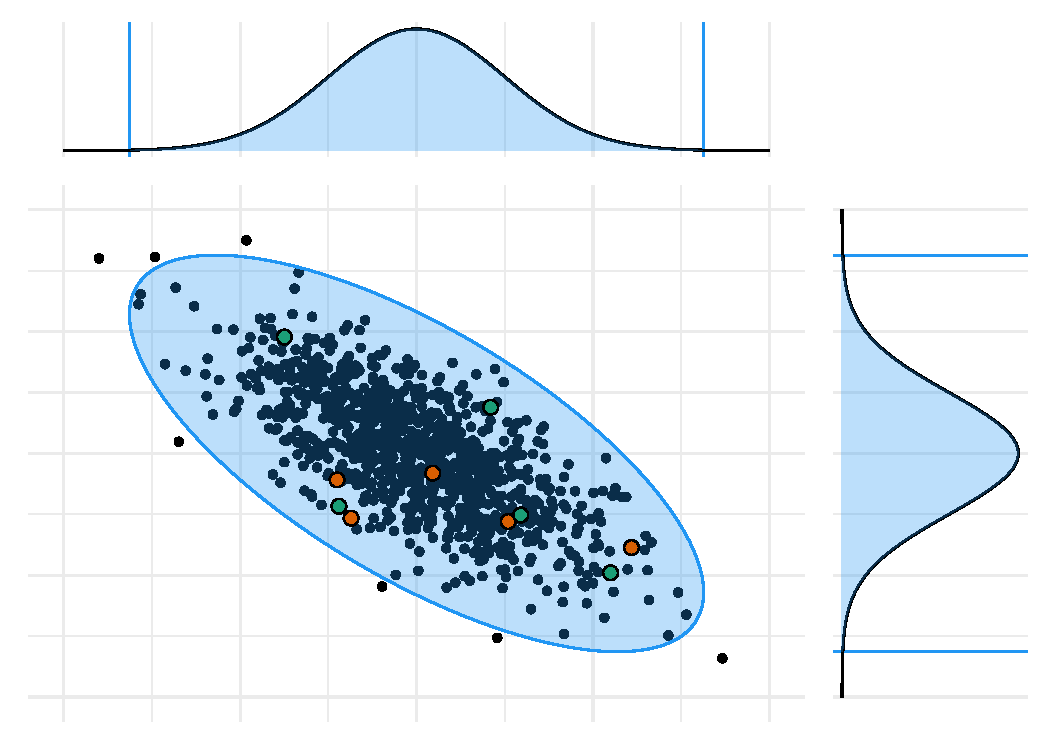
\includegraphics[width=0.8\linewidth]{img/slides/several_points.pdf}}
        \onslide<3->{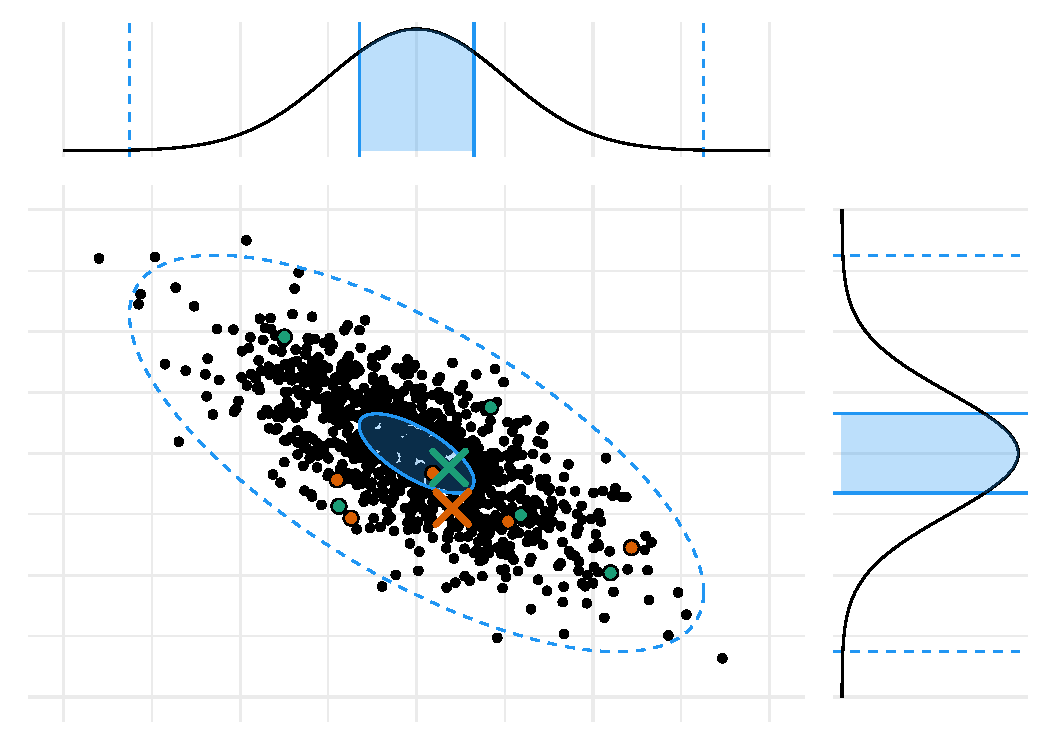
\includegraphics[width=0.8\linewidth]{img/experiment/non_regression/statistics/several_points.pdf}}
    \end{center}
\end{frame}

\begin{frame}{Result: performance fluctuation}
    \begin{center}
        \begin{minipage}[t][.4\textheight][t]{\textwidth}
            Performance fluctuation of the node dahu-14 (5-day window)\\
            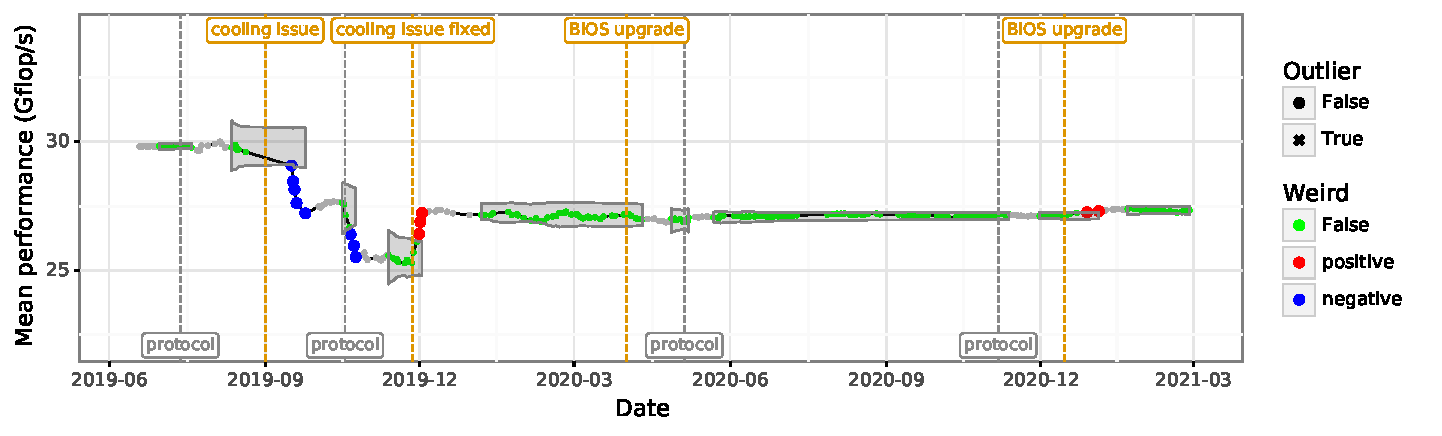
\includegraphics[width=0.9\linewidth]{img/slides/evolution_dahu-14_windowed.pdf}
        \end{minipage}
        \begin{minipage}[t][.4\textheight][t]{\textwidth}
            Performance fluctuation of the node dahu-32 (5-day window)\\
            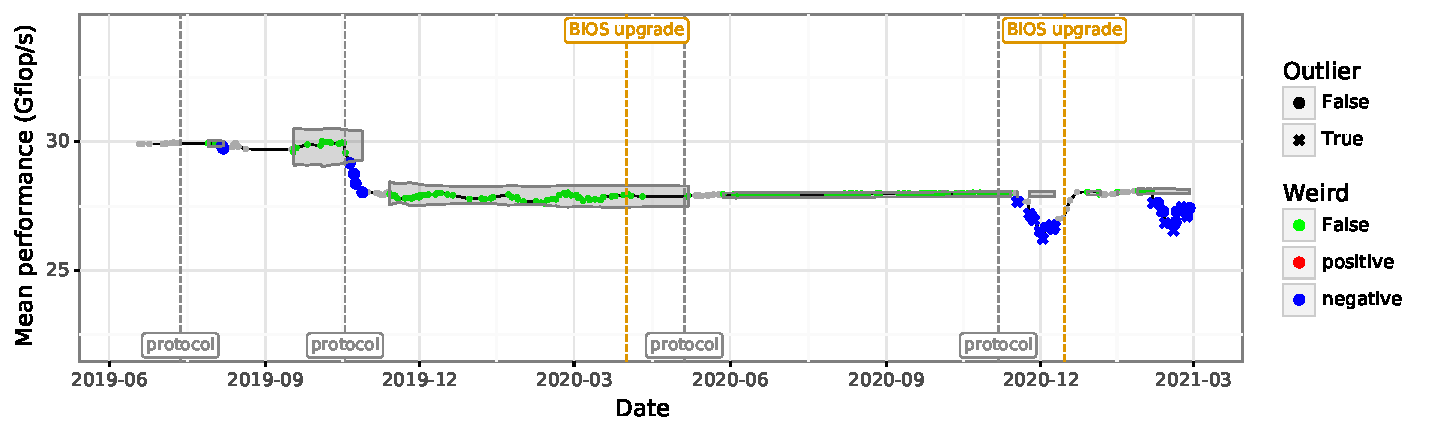
\includegraphics[width=0.9\linewidth]{img/slides/evolution_dahu-32_windowed.pdf}
        \end{minipage}
    \end{center}
\end{frame}

\begin{frame}{Result: performance overview}
    Overview of the performance on cluster dahu \uncover<2>{(5-day window)}\\
    \begin{center}
        \includegraphics<1>[width=0.9\linewidth]{img/slides/overview_dahu.pdf}
        \includegraphics<2>[width=0.9\linewidth]{img/slides/overview_windowed_dahu.pdf}
    \end{center}
\end{frame}

\begin{frame}{Performance tests: wraping up}
    Multi-variable test also implemented, on all the model coefficients
    \pause

    Results available at \alert{\url{https://cornebize.net/g5k\_test}}

    \begin{minipage}{0.55\linewidth}
        \fbox{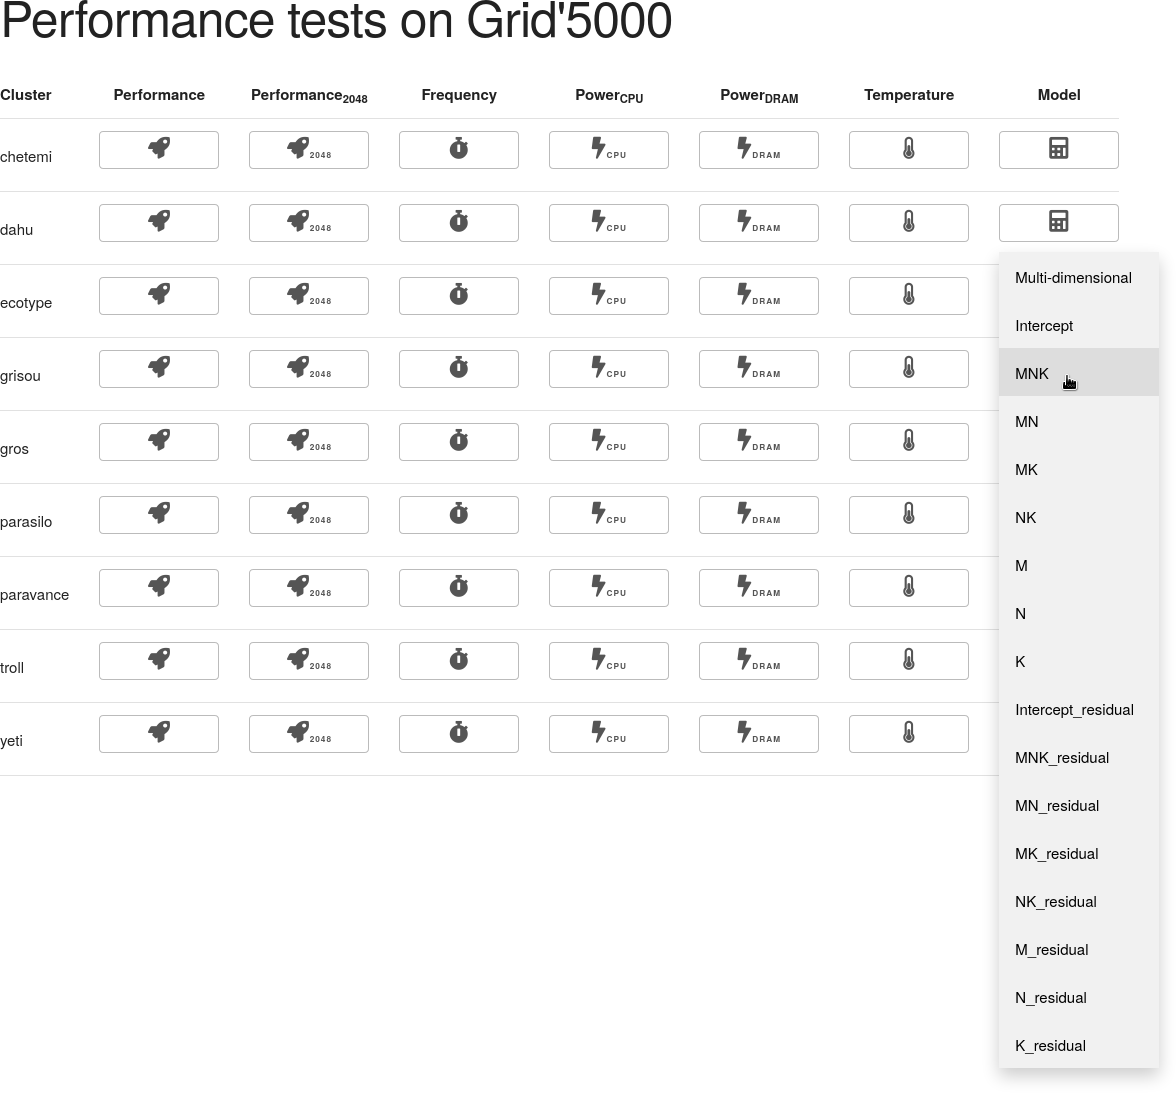
\includegraphics[width=\linewidth]{img/experiment/non_regression/implementation/g5k_test_home.png}}
    \end{minipage} \hfill\pause%
    \begin{minipage}{0.4\linewidth}
        \begin{block}{Detected events}
            \begin{itemize}
                \item BIOS upgrades
                \item Cooling issue
                \item Faulty memory
                \item Power instability
            \end{itemize}
            \pause

            All went unnoticed by both Grid'5000 staff and users, despite significant effects

            \alert{\(\Rightarrow\) Great help potential}
        \end{block}
    \end{minipage}
\end{frame}

\section{Concluding thoughts}

\begin{frame}{Can we trust our predictions?}
    How to know if our predictions are faithful?

    There is no \emph{correctness proof}, a model can be validated only by \alert{trying to break it}

    \pause \medskip
    \(\Rightarrow\) Often broke the simulations during the last few years

    \pause
    \alert{Repeated} the whole study \alert{from scratch} on a new cluster:~~~\alert{\textbf{\Huge \checkmark}}

    Where to stop? Try all the Grid'5000 clusters? Other applications?
\end{frame}

\begin{frame}{There is no planet B}
    About \NSI{18}{\tonne} of CO2eq were emitted for this thesis

    \begin{minipage}{0.38\linewidth}
        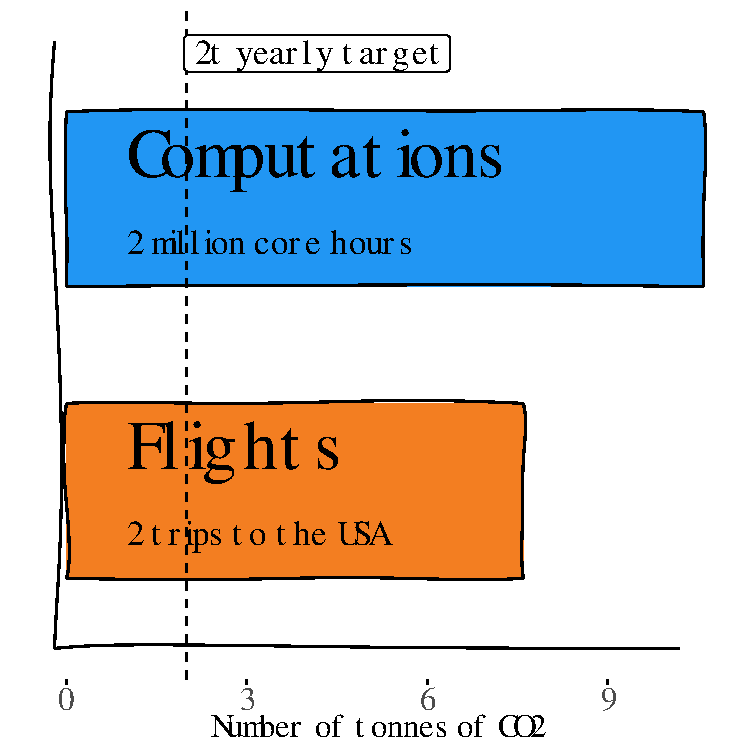
\includegraphics[width=\linewidth]{img/slides/co2.pdf}
    \end{minipage} \hfill\pause%
    \begin{minipage}{0.6\linewidth}
        Do we really \emph{need} to attend conferences in person?
        \medskip

        What about computations?
    \end{minipage} \hfill
\end{frame}

\begin{frame}{Why so many computations?}
    More than half the total core hours were used for performance tests
    \pause
    \begin{block}{How to reduce them?}
        \begin{itemize}
            \item Change the experiment procedure (\eg no full node reinstallation)
            \item Test less frequently (\eg only once a week)
            \item Use a cheaper test (\eg shorter warmup, less extensive coverage)
        \end{itemize}
    \end{block}
    \pause
    \begin{block}{Who should be responsible of tests?}
        \begin{itemize}
            \item Platform staff? But what should they test?
            \item Researchers? Isn't it redundant?
        \end{itemize}
    \end{block}
\end{frame}

\begin{frame}{Perspectives}
    Applying our approach on the whole life cycle of supercomputers:
    \begin{description}
        \item[Design] Constructing the best machine for a given budget, using co-design
        \item[Scheduling] Using predictions to improve the decisions of schedulers
        \item[Development] Debugging and improving software performance
        \item[Maintenance] Ensuring that routine upgrades keep the performance as expected
    \end{description}
\end{frame}

% See:
%   https://academia.stackexchange.com/a/88068/37904
%   https://unix.stackexchange.com/a/277987/106103
%   https://stackoverflow.com/a/5349842/4110059
\begin{frame}[plain]
    \centering
    \setlength{\tabcolsep}{0pt}
    \renewcommand{\arraystretch}{0}
    \begin{tabular}{|c|c|c|}
        \hline
        \addframe{27}  & \addframe{29}  & \addframe{34}  \\
        \hline
        \addframe{39}  & \addframe{41}  & \addframe{47}  \\
        \hline
        \addframe{62}  & \addframe{64}  & \addframe{70}  \\
        \hline
        % Some ugly stuff, it would be great to find something better...
        \vspace{10pt}\\
        \multicolumn{3}{c}{Thank you all!}\\
    \end{tabular}
\end{frame}

\end{document}
